\documentclass[a4paper,twoside, 12pt]{article}
% Brug denne, hvis der kun printes på den ene side!
%\documentclass[a4paper]{article}
\usepackage[utf8]{inputenc}
\usepackage{amsmath}
\usepackage{amsfonts}
\usepackage{amssymb}
\usepackage[english]{babel} 
\usepackage{graphicx}

\usepackage{color}
\usepackage{wrapfig}
\usepackage{fancyhdr}
\setlength{\headheight}{15pt}
\usepackage{url}
\usepackage{caption}
\usepackage{pgfplots}
\usepackage{tikz}
\usetikzlibrary{patterns}
\usepgfplotslibrary{fillbetween}
\usepackage{listings}

\usepackage{enumitem}
\usepackage{caption}
\usepackage{subcaption}
\usepackage{multirow}
\usepackage{hyperref}
\usepackage[official]{eurosym}
\usetikzlibrary{patterns}

\pgfplotsset{compat=1.14}

\usepackage[rmargin=3.2cm,tmargin=3.5cm]{geometry}

\setlength{\parindent}{0pt}
\setlength{\parskip}{1ex plus 0.5ex minus 0.2ex}
%Nu laver vi lige en header
\pagestyle{fancy}
\fancyhf{}
\rhead{Markus Greve Bech}
\lhead{Deep indoor measurements for narrownband-IoT}
\rfoot{Page \thepage}

%\pgfplotsset{compat=1.15}

\begin{document}

\begin{titlepage}
\pagenumbering{gobble}
\centering

\vspace*{\stretch{1}}

\rule{\textwidth}{1mm}\\
\vspace{1cm}
\Huge\bfseries Deep indoor measurement for NB-IoT\\
\vspace{0.7cm}
\rule{\textwidth}{1mm}\\
\vspace{3cm}
\large by\\
Markus Greve Bech (s144065) \\

\vspace*{\stretch{2}}
\normalsize
\begin{flushleft}
Manual for project on Deep indoor measurement for NB-IoT\\
Technical university of Denmark\\
8th of February 2019
\end{flushleft}
\end{titlepage}
\thispagestyle{plain}

 \newpage
\tableofcontents
\thispagestyle{plain}
\newpage
\pagenumbering{arabic}

\section{Purpose}
Mapping signal strength for NB-IoT gives an idea of how to best make use of IoT devices. Since IoT devices depends on connectivity to the internet, placing such a device in a location without sufficient signal to connect, would be infeasible. 

To map indoor signal strength of NB-IoT a setup with two LIDAR sensors and an antenna is used to find indoor positions as well as signal strength. The two LIDAR sensors are controlled by an arduino while the antenna is controlled by a Rohde and Schwarz TSMW Universal Rodio Network Analyzer. By capturing measurements while moving, indoor placement can be related to signal strength.


\section{Manual}
The following describes how to used the test setup. You will need:
\begin{itemize}
	\item \textbf{Digital resources:}
	\begin{itemize}
		\item The \texttt{i2c\_scanner.ino} arduino script.
		\item The \texttt{Lidar.ino} arduino script.
		\item The \texttt{I2C\_Rev5.zip} library for arduino.
		\item The \texttt{LidarLite\_Arduino\_labrary-master.zip} library for arduino.
		\item The \texttt{arduinoTest.m} Matlab script.
		\item The \texttt{readDistance.m} Matlab script.
		\item The \texttt{takeRange.m} Matlab script.
		\item The \texttt{waitForBusy.m} Matlab script.
		\item The \texttt{GPSmapping.m} Matlab script.
		\item The \texttt{lldistkm.m} Matlab script.
		\item The \texttt{simple\_kml\_writer.m} Matlab script.
		\item The \texttt{get\_power\_measurements.m} Matlab script.
		\item The \texttt{postprocess.m} Matlab script.
		\item Installed and running MATLAB R2018b.
		\item Installed and running MATLAB R2015a.
		\item Installed and running Arduino Software (IDE).
	\end{itemize}
	\item \textbf{Physical resources:}
	\begin{itemize}
		\item The arduino board with the two LIDAR sensors attached. 
		\item Laptop with all the digital resources on.
		\item Powersource (a car battery with the suitable adapter).
		\item Rohde \& Schwarz TSMW Universal Radio Network Analyzer.
		\item Means of fastening (a metal plate and clamps or similar).
		\item A trolley or simiar, that can support the equipment.
	\end{itemize}
\end{itemize}
All the scripts can be found in the github repository: \\
\url{https://github.com/MonsterMarkus/NB-IoT-indoor-measurements}.

\subsection{Record metadata}
Before starting a proper scenario must be chosen. Scenarios are further explained in section \ref{sec:scenarios}. The recordings of metadata is done by writing all metadata in directly in the matlab script \texttt{arduinoTest.m}. Here the \texttt{metaData} struct must be updated to fit the scenario. These informations are later stored in a \texttt{.mat} format.

\subsection{Setup}
To setup a measurement follow the steps below accordingly:
\begin{itemize}
	\item Start the Arduion IDE.
	\item Make sure that Tools$\rightarrow$Board is set to Arduino Mega 2560
	\item Install the \texttt{.zip} libraries (Sketch$\rightarrow$Include library$\rightarrow$Add .ZIP library...). (Only for the first setup)
	\item Disconnect one of the LIDARs (the blue and green wire)
	\item Run \texttt{i2c\_scanner.ino}, changing the address of the connected one from the default \texttt{0x62} to \texttt{0x61}. By opening the serial monitor (found under tools) and setting the baud rate to 9600, the connected components addresses can be identified.
	\item Now connect the other LIDAR to the board.
	\item The other LIDAR should now be connected and have address \texttt{0x62}.
	\item Run the \texttt{Lidar.ino} now. To ensure it works, open the serial monitor and change the baud to 115200 and follow the instructions. This step is not always mandatory, but on some systems a necessity to enable the matlab script. 
	\item Close the serial monitor.
 	\item Set up the equipment on a rolling table or similar. An example sketch can be seen in figure \ref{fig:setup}.
\end{itemize}
\begin{figure}[ht]
\centering
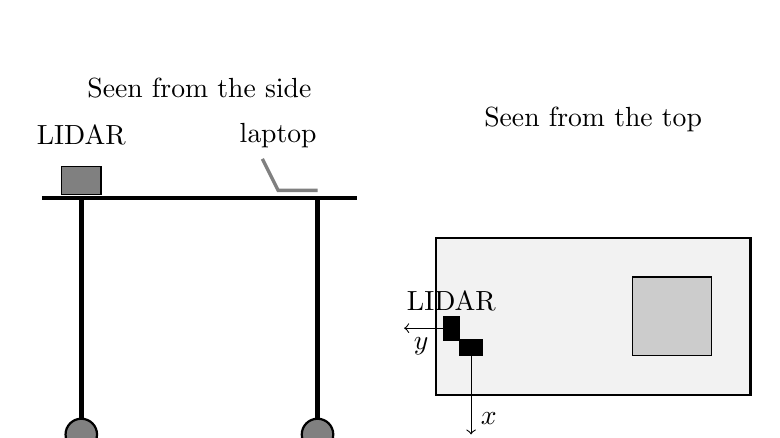
\begin{tikzpicture}
	%Seen from the side
	\node[] at (2,4.4) {Seen from the side};
	%Table on wheels
	\draw[ultra thick] (0,3)--(4,3);
	\draw[ultra thick] (0.5,3)--(0.5,0);
	\draw[ultra thick] (3.5,3)--(3.5,0);
	\filldraw[fill = gray, thick] (0.5,0) circle (0.2);
	\filldraw[fill = gray, thick] (3.5,0) circle (0.2);
	%laptop
	\draw[gray, very thick] (2.8,3.5)--(3,3.1)--(3.5,3.1);
	\node[] at (3,3.8) {laptop};
	%LIDAR
	\filldraw[fill=gray] (0.25,3.05) rectangle (0.75,3.4);
	\node[] at (0.5,3.8) {LIDAR};
	
	%seen from the top
	\node[] at (7,4) {Seen from the top};
	%Table
	\filldraw[fill=gray!10!white!, thick] (5,0.5) rectangle (9,2.5);
	
	%laptop
	\filldraw[fill = black!20!white] (7.5,1) rectangle (8.5,2);
	
	%LIDAR
	\filldraw[fill = black] (5.1,1.2) rectangle(5.3,1.5);
	\filldraw[fill = black] (5.3,1) rectangle (5.6,1.2);
	\node[] at (5.2,1.7) {LIDAR};
	%axis
	\draw[->] (5.1,1.35)--(4.6,1.35);
	\node[anchor=north west] at (4.6,1.35) {$y$};
	\draw[->] (5.45,1)--(5.45,0);
	\node[anchor=south west] at (5.45,0) {$x$};	
	
\end{tikzpicture}
\caption{Example setup.}
\label{fig:setup}
\end{figure}

To setup the TSMW box, simple connect it to the power source and connect it with a LAN cable to the computer. When the measurements is to be carried out, run the \texttt{get\_power\_measurements.m} script and terminate by pressing \texttt{ctrl+c}.

Pictures of the setup can be seen in figure \ref{fig:rul1}.

\begin{figure}[ht]
\centering
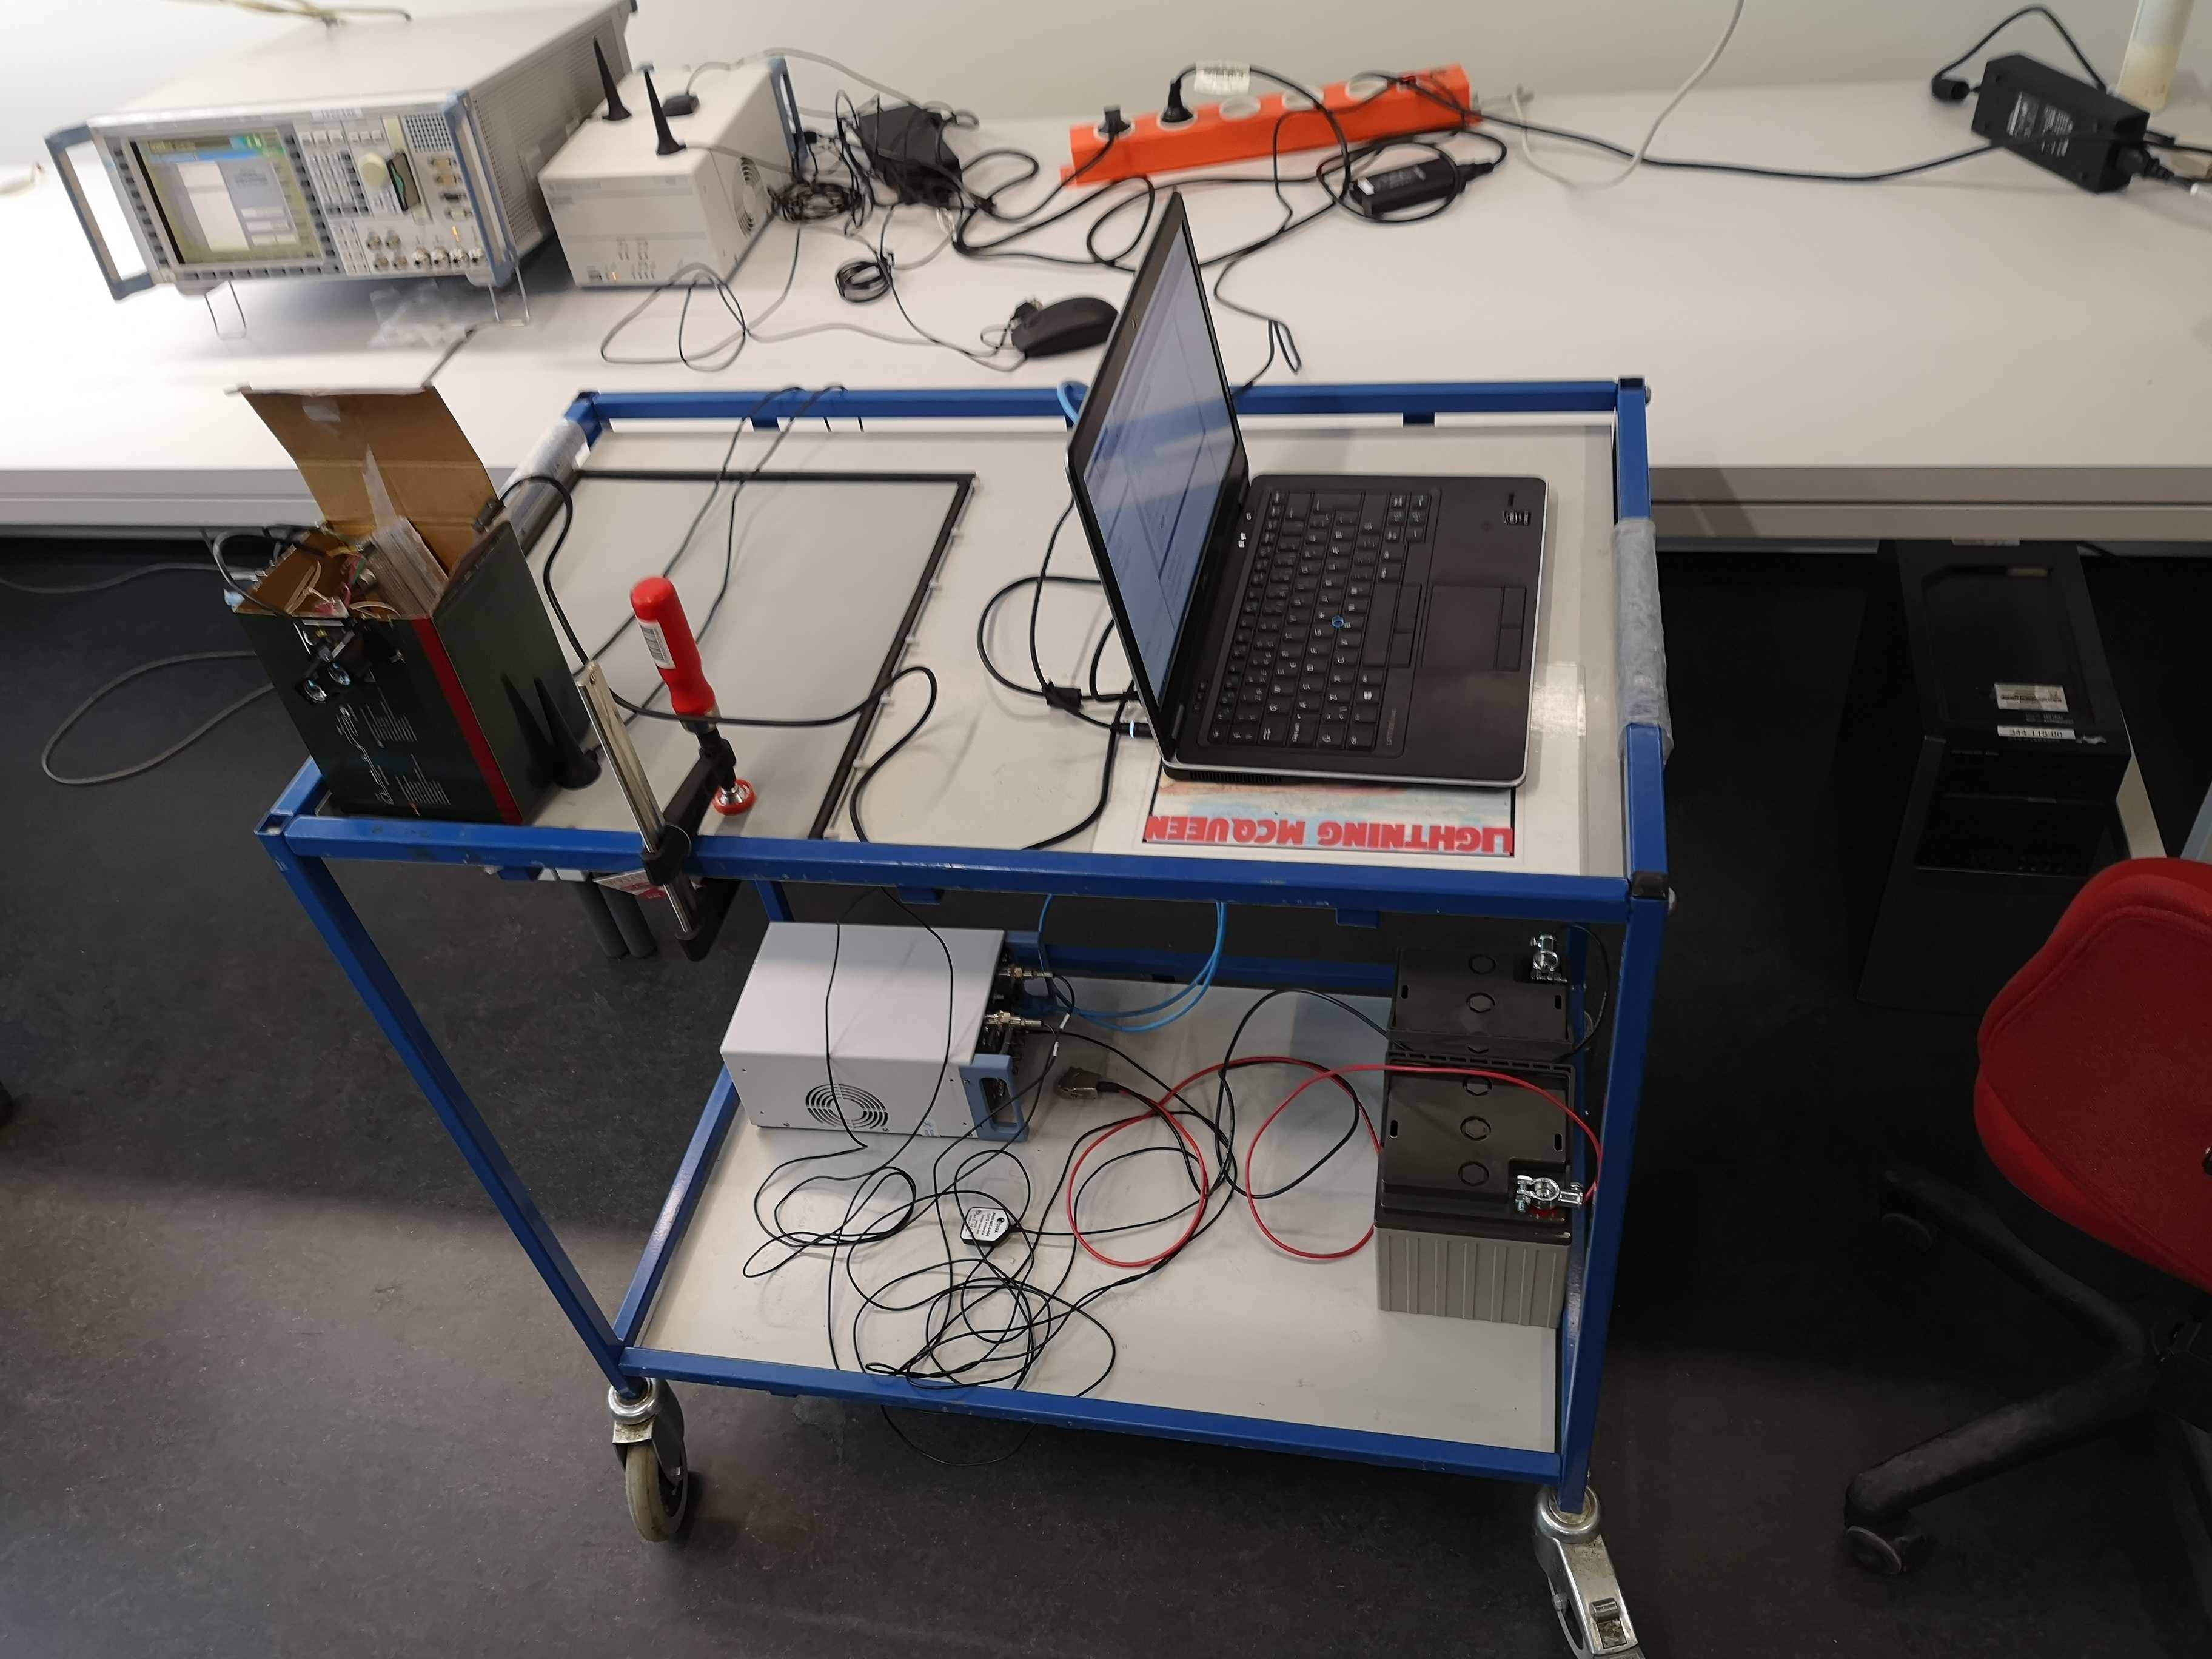
\includegraphics[width=0.4\textwidth]{rullebord1.jpg} \quad 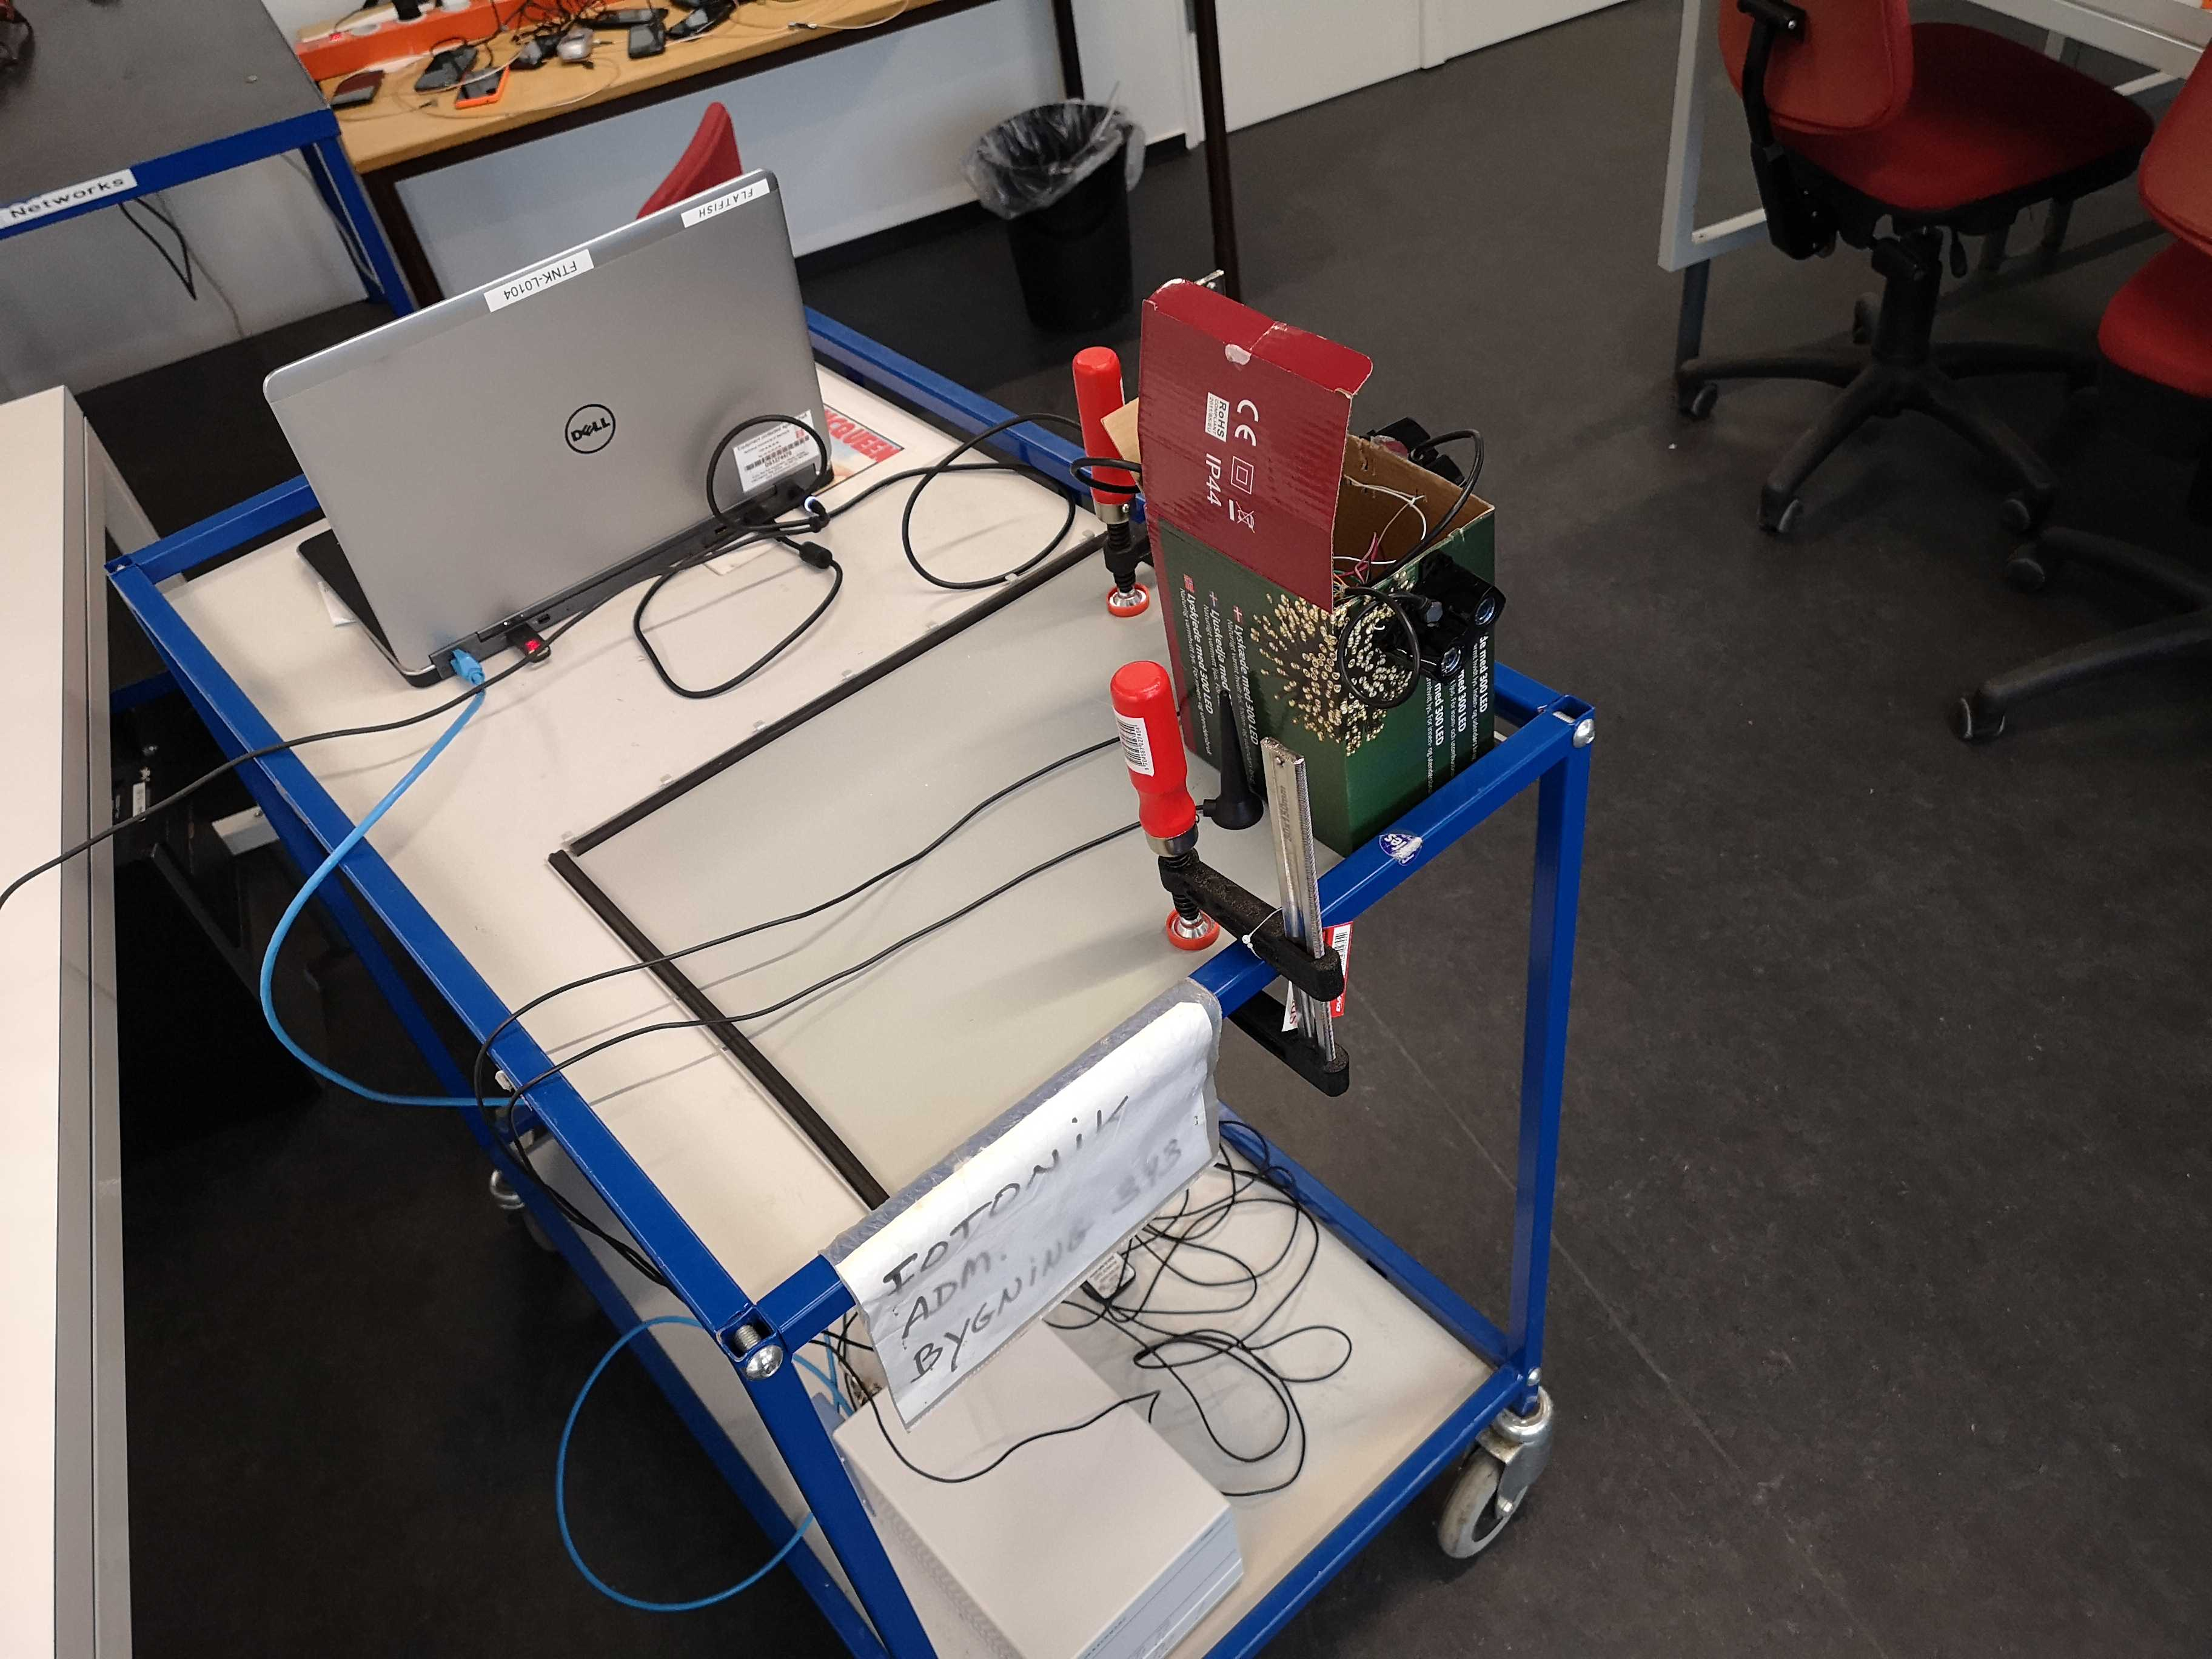
\includegraphics[width=0.4\textwidth]{rullebord2.jpg}
\caption{Pictures of the setup from the 25th of January.}
\label{fig:rul1}
\end{figure}


\subsection{Recording}

To record data, perform the setup procedure, place yourself in the desired location and run the matlab script \texttt{arduinoTest.m} in the R2018b release. The 2015a release can then used to run the \texttt{get\_power\_measurements.m}. To stop the arduino press any bottom and to stop the TSMW use \texttt{ctrl +c}. While recording move around slowly and controlled. In \cite{artikel} it is proposed to have a grid of 0.5m by 0.5m at a height of 2m above the floor. While the height depends on the specific setup, the movement can be done freely and thus is a 0.5m seems reasonable. The pattern could be done in a "lawnmover" style as shown in figure \ref{fig:lawnmover}.
\begin{figure}[ht]
\centering
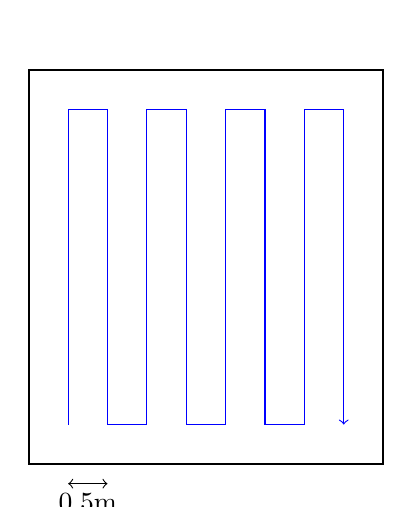
\begin{tikzpicture}
	\draw[thick] (0,0) rectangle (4.5,5);
	\draw[color =blue,->] (0.5,0.5)--(0.5,4.5)--(1,4.5)--(1,0.5)--(1.5,0.5)--(1.5,4.5)--(2,4.5)--(2,0.5)--(2.5,0.5)--(2.5,4.5)--(3,4.5)--(3,0.5)--(3.5,0.5)--(3.5,4.5)--(4,4.5)--(4,0.5);
	\draw[<->] (0.5,-0.25)--(1,-0.25);
	\node[anchor=north] at (0.75,-0.25) {0.5m};
\end{tikzpicture}
\caption{Proposed movement pattern. The "lawnmover" style makes it easy to remember to map the entire room.}
\label{fig:lawnmover}
\end{figure}

Furniture and people moving around in a room disturbs the measurements. To avoid furniture and most people the sensors could be raised to 2m or above, while keeping the antenna at the same height or moving it up. Remeber to note it in the metadata.

\subsection{Postprocessing}
As the data from the LIDAR sensors is saved to a \texttt{.mat} file, all one would have to do is to run the\texttt{GPSmapping.m} function with the proper filename. Then two sets of plots are made for a quick sanity check and then the GPS coordinates (in decimal degrees) and a \texttt{.kml} file is saved. The power measurements are also loaded and mapped to the positions utilizing timestamps. For the function to work, two GPS coordinates are needed as reference. One to map the origin and another one to map the angle of the wall. An illustration of how two GPS coordinates helps map a room can be seen in figure \ref{fig:map}. To find GPS coordinates, google map is here used and google earth is used to plot the measured coordinates. The GPS coordinates are manually written into the script. The GPS Coordinates used in the following examples are all found using google maps and estimating a position based on satellite pictuers. 

The \texttt{postprocess.m} function called from within the \texttt{GPSmapping.m} script removes any surplus measurements. As of this moment only an extensive amount of TSMW measurements are handled. The power measurements are related to the position by taking the measurements closest in time and adding the mean of those as the recieved power.

\begin{figure}[ht]
\centering
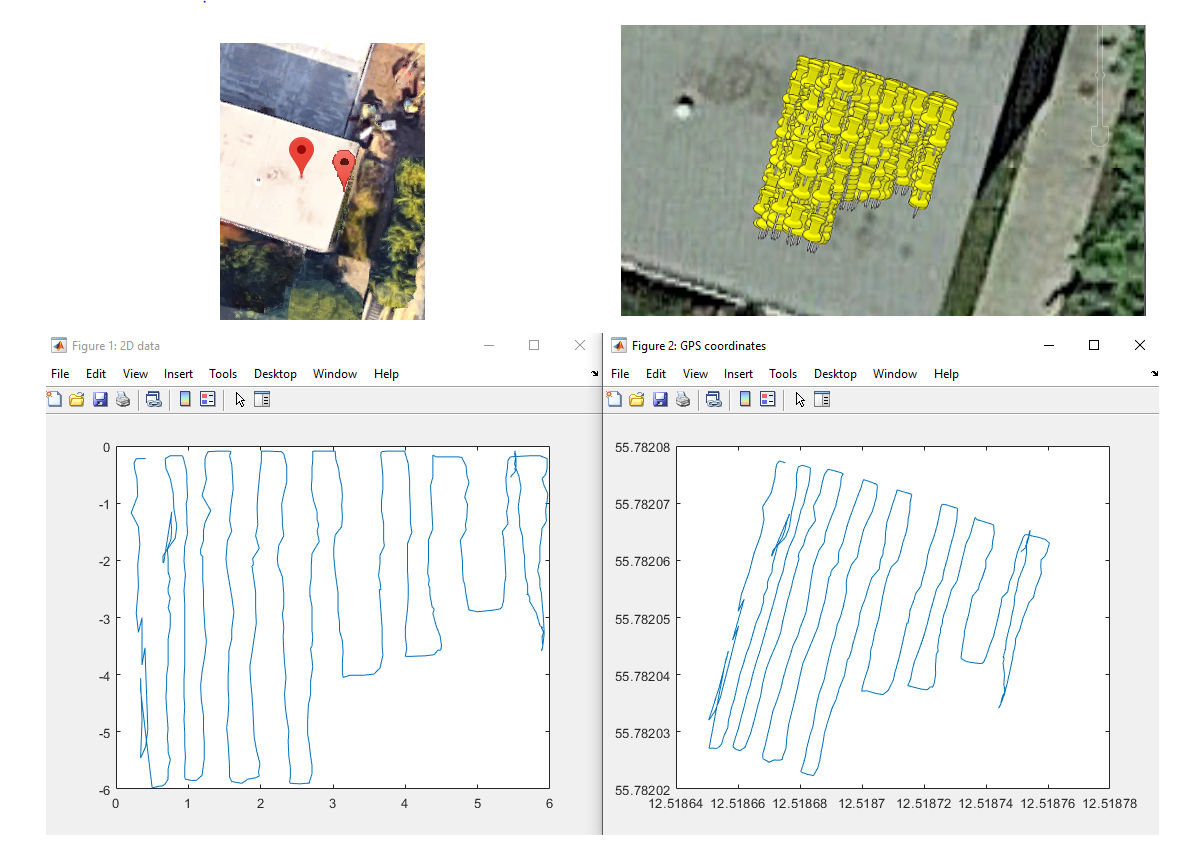
\includegraphics[width=\textwidth]{plotexample.png}
\caption{Example of mapping from 2D to GPS. The GPS coordinates are found by using google maps.}
\label{fig:map}
\end{figure}


\subsection{Errors}
Errors will happen and they can easily be removed if identified. When approaching the 40m limit the sensors are prone to output 0cm instead of the actual distance, espicially if the surface is glass. This can be solved by removing all samples of 0cm. Also if the difference in distance suddenly changes a lot, for example due to a collegue walking by or an overlooked piece of furniture, that measurement could be removed as all movement should be slow and smooth. However when walking through a door or similar, the measured distances will rapidly change. In general avoid glass as the measurements jumps between the actual distance and the distance plus around 3m.

As of this moment, these errors are not automatically correted when post processing.

\section{Scenarios}\label{sec:scenarios}
To best map the signal quality in terms of position a number of scenarios will have to be adressed. In \cite{artikel} a parking lot, with 4 floors including ground floor, is examined. Besides varyring the floor, the line of sight is also varyed by having different transmitters. With a range limit of less than 40m, large "open" indoor areas are hard to map. The following is a list of possible scenarios and combinations of these can be used to map the signals indoor. 
\begin{itemize}
	\item Floors
	\begin{itemize}
		\item -2nd to 3rd floor.
	\end{itemize}
	\item LOS
	\begin{itemize}
		\item LOS
		\item NLOS
		\item no LOS
	\end{itemize}
	\item Walls, material
	\begin{itemize}
		\item Wood
		\item Bricks
		\item Concrete
		\item Glass - thermo windows, double layer, etc.
		\item Other building materials.
	\end{itemize}
	\item Walls, layers
	\begin{itemize}
		\item 1-10 Layers
	\end{itemize}
\end{itemize}

By examening all these scenarios a more complete understaning of how to predict signal quality indoors could be achieved. Finding suitable and compareable rooms is a necessity for this to happen. 


\subsection{Getting above 40m}
As the LIDAR is limited to 40m, a solution to this has to be found to map hallways corretly. The ideas at the moment include the following:
\begin{itemize}
	\item Place a piece of cardboard (or similar) for each 40m and add that as an offset between measurements. Remember to do it in the right direction. This would also make it possible to map larger rooms, by dividing it into smaller parts and mapping those.
	\item Only do a few refference measurements in the hallways with manual input.
\end{itemize}

\subsection{Glass}
When measurering the distance to a wall/window of glass, the LIDARs adds around 3m sometimes and sometimes not. It is very uncertain and not recommended to do distance mesurements up against a glass wall/window.




\section{Results}
By comparing timestamps of the TSMW and arduino measueremnets the results can visualized as showed in figure \ref{fig:databar} and \ref{fig:basementEast}. A simple postprocessing script extracted the measured power and distance and connected the two with the timestamps, such that a single point had the mean of 600ms ($\pm$ 300ms) of power measurements associated. By rotation the position measurements and inverting their axis the movement can be mapped to a displacement in GPS coordinates and as such is the results produced.

As one can see from the figures (\ref{fig:databar} and \ref{fig:basementEast}), the signal strength drops close to the walls and are "best" in the middle of the rooms. 

\begin{figure}[ht]
\centering
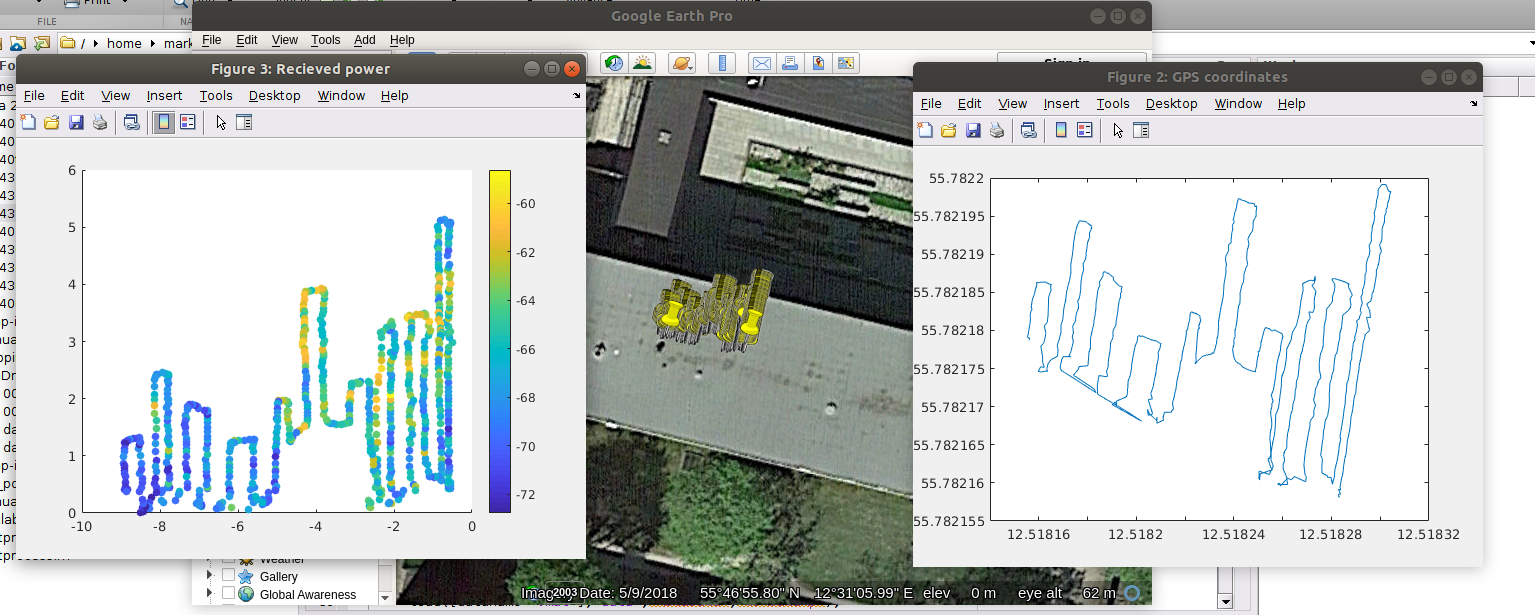
\includegraphics[width=0.8\textwidth]{databar.png}
\caption{Measurements from the inside the databar, room 009 in building 343. The room had a lot of furniture, making a complete coverage mapping of the room inpractical with the simple setup. The signal quality drops as one moves closer to the walls and further away from the windows. The databar is located at the north side of the building and is thus closer to the transmitter compared to the measurement done on the south side of the building such as the ones described in figure \ref{fig:basementEast}. Still LOS is not achieved as building 340 is blocking. The displayed power is in dB.}
\label{fig:databar}
\end{figure}

\begin{figure}[ht!]
\centering
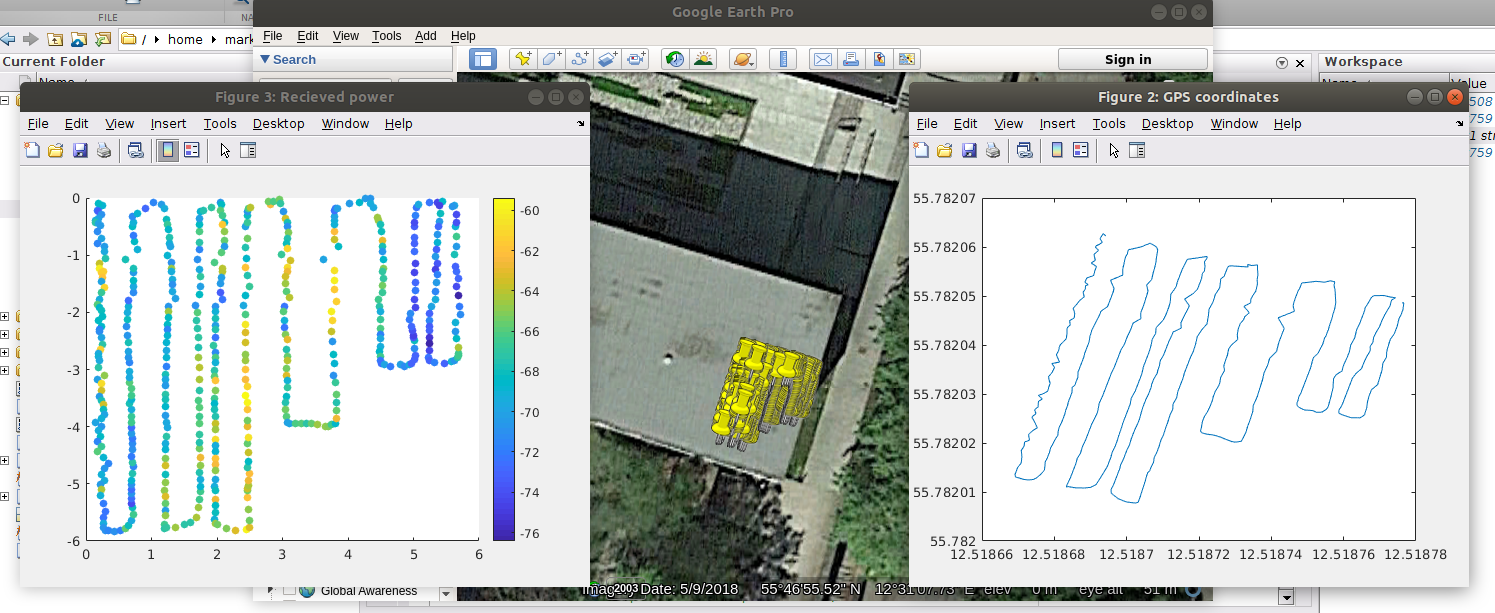
\includegraphics[width=0.8\textwidth]{stairs.png}
\caption{Measurements from the basement at the stairs in the east end of 343. When moving closer the the west wall or under the stairs to the east, the signal is weakned, while in the middle it is at its best. In the middle there is free space all the way up as the stairs revolve around some free space. These measurements are closest the the southern wall and thus further away from the transmitter to the north compared to the measurements described in figure \ref{fig:databar}. The displayed power is in dB.}
\label{fig:basementEast}
\end{figure}

As the measurements are dependent on smooth walls, no glass walls and prefereably no furniture or people, finding easy-to-map rooms prooved difficult. Thus is the resulting measurements somewhat uneven. Furthermore is the size of the rolling table a limiting factor as to which corners can be entered as the entire table has to be able to fit. The table also hindered wall to wall measurements, since the extent of the table were larger that the entire setup (see figure \ref{fig:rul1}).

Some of these limitation could be reduced by introducing a diffrent setup. The LIDAR sensors and the antennas is not required to be at same altitude and a setup with the LIDAR sensors elevated to a heigth above furniture, possibly on a smaller rolling table (or similar) would improve the agility and mapping robustness of the setup. 

In terms of precision in relating the measured positions to GPS coordinates, other methods should be considered. For the measurements shown in figure \ref{fig:databar} and \ref{fig:basementEast} the corresponding refference point and the callibration points (for calculating the angle relative to north) are found by estimating a position on google maps and sanity checking it, by plotting in google earth. A more solid (and faster) approach could be to use the GPS module of TSMW to find a starting point. The GPS will not work while indoor, but by placing it at a known distance to the LIDAR an offset can be added to the measurements and provide more accurate mapping.
 
 
\section{Uncertanties}
There are some uncertanties to take into account. The most relevant are found here.
\begin{itemize}
	\item Height above ground, measured with ruler $\pm$0.5cm
	\item The GPS reference coordinates. As long as it is done by point and click on google maps there is an potential uncertainty of several meters. This can be minimized be having a reference measurement of the GPS position out of a window or door as a refference. 
	\item Wether or not LOS or NLOS is achieved is also quite unsure. Fair estimates can be made from calculating the fresnel zone and investigating the terrain.
	\item When adding an offset, if measured with a ruler an uncertainty of $\pm$0.5cm is likely.
	\item If the angle of the LIDAR sensors change, the uncertainty is large. By change the angle $\theta$ slightly the measured distance $x'$ becomes $\frac{x}{\cos \theta}$ instead of $x$.
\end{itemize}
To asses the measured values more accurately these uncertainties should be handled in a suitable manner. The uncertainties of the signal measurements should also be taken into account.

Since the transmissions for NB-IoT follows the LTE frame structure, resources are assigned on a ms scale, while the measurements are performed in a 10ms scale. The lower sample rate leads to uncertainties wether or not a signal was assigned for each measurement and thus may a power measurement be a mean of both empty and full slots.

\section{Conclusion}
By using the described test setup, indoor measurements relating signal power of NB-IoT and position can be carried out. To map an indoor location to GPS coordinates estimates can give a fair idea, but actual measurement would improve accuracy. The setup has the potential to execute deep indoor measurements of NB-IoT in a number of cases, but has some limitations. Some limitations, such as range, can be omitted without much effort, while others require more extensive measures, like handling glass walls and/or uneven walls etc.

By reasonable postprocessing, measurements can be illustrated and exported. The measurements shows stronger signal in the middle of a room compared to the walls, which are further away from the transmitter.



\clearpage
\newpage
\bibliography{mybib}
\bibliographystyle{unsrt}


\end{document}